\chapter{Exemples de communication entre agents avec JASON}
\section{Environnement de travail}
\paragraph{}
L'IDE de la plateforme JASON est jEdit, il se présente comme tout IDE classique avec les fonctionnalités adéquates pour la manipulation des agents et des architectures BDI.
\begin{figure}[H]
	\centering
	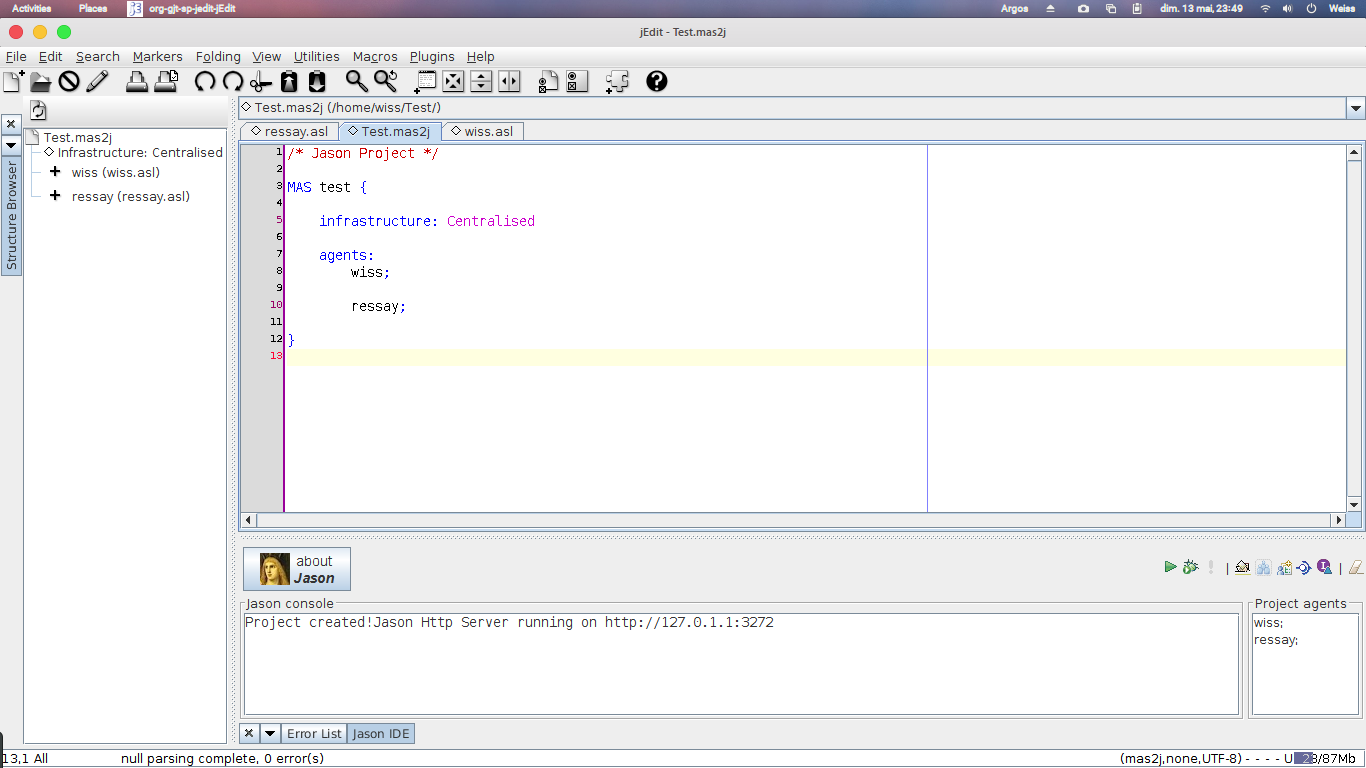
\includegraphics[width=\textwidth]{imgs/jEdit.png}
	\caption{Fenêtre d'édition de l'IDE jEdit}
\end{figure}
\newpage
\section{Inférence locale}
\paragraph{}
Un agent dans JASON peut utiliser l'architecture BDI pour lancer son propre moteur d'inférence, prenons l'exemple suivant : \\
\begin{itemize}[label=\textbullet]
	\item l'agent a une croyance initiale que la saison est l'été.
	\item il ajoutera la croyance article(tshirt) si la saison est l'été en exécutant le plan : sayTshirt.
\end{itemize}

\paragraph{}
le code est le suivant : \\
\begin{figure}[H]
	\centering
	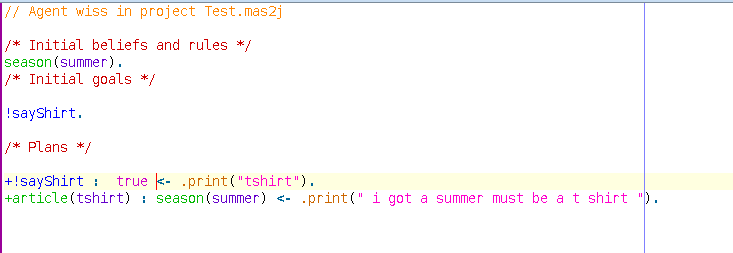
\includegraphics[width=0.8\textwidth]{imgs/jasonWiss.png}
	\caption{Code agentSpeak de l'agent wiss}
	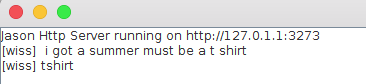
\includegraphics[width=0.8\textwidth]{imgs/jasonWissDone.png}
	\caption{résulat}
\end{figure}
\section{Scénario simple de communications}
\paragraph{}
Le scenario est le suivant : 
\begin{itemize}[label = \textbullet]
	\item l'agent Ressay envoie un message a l'agent Wiss lui disant que l'article est tshirt.
	\item l'agent Wiss attendra un message de la part de Ressay seulement car il l'a marqué comme étant fiable.
	\item Wiss ré-exécute l'inférence du scénario précédent.
\end{itemize}

\begin{figure}[H]
	\centering
	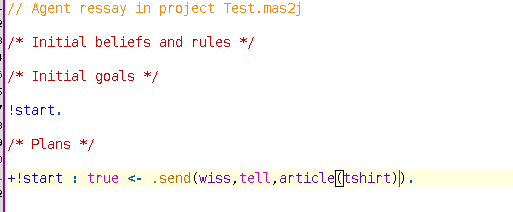
\includegraphics[width=0.8\textwidth]{imgs/jasonRessay.png}
	\caption{Ressay envoie le message}
	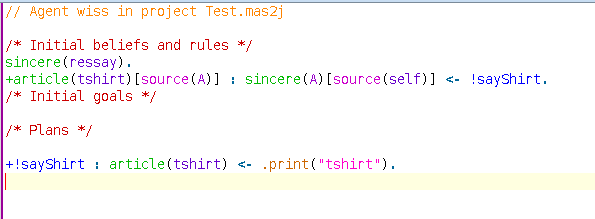
\includegraphics[width=0.8\textwidth]{imgs/wissRecievedRessay.png}
	\caption{Wiss reçoit}
	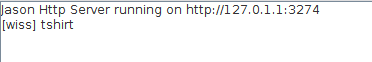
\includegraphics[width=0.8\textwidth]{imgs/wissRessayDone.png}
	\caption{Résultat}
	
\end{figure}
